% TEX compiler = xelatex
% copyright arturo salinas-aguayo 2024
\documentclass[12pt]{article}

\usepackage{graphicx}
\usepackage{amsmath}
\usepackage{array}
\usepackage{fontspec}
\usepackage{unicode-math}
\usepackage{sim-os-menus}
\usepackage{xfp}
\usepackage{amsfonts}
\usepackage{fancyhdr}
\usepackage{geometry}
\usepackage{circuitikz}
\usepackage{subfigure}
\usepackage{caption}
\usepackage{karnaugh-map}
\usepackage{bm}
\usepackage[table]{xcolor}
\usepackage{float}
\usepackage{subcaption}
\setmainfont{Berkeley Mono Nerd Font}
\setmonofont{Berkeley Mono Nerd Font}
\setmathfont{Berkeley Mono Nerd Font}

\geometry{letterpaper, margin=1in}
\graphicspath{ {../images/} }

% Header and Footer
\pagestyle{fancy}
\fancyhf{}
\fancyhead[L]{CSE 2301 - Lab 12: VHDL}
\fancyhead[R]{\thepage}
\setlength{\headheight}{15pt}

\author{Arturo Salinas-Aguayo}
\title{Lab 12: VHDL}
% theorem set
\newtheorem{example}{Example}
% Example block environment
\newenvironment{examp}
{
	\vspace{.5cm}
	\hrule
\begin{example}\upshape}
	{\hrule
		\vspace{0.5cm}
\end{example}}

\begin{document}
\newcommand{\closure}[2][3]{%
	{}\mkern#1mu\overline{\mkern-#1mu#2}}
\newcommand\ncoverline[1]{\mkern1mu\overline{\mkern-1mu#1\mkern-1mu}\mkern1mu}
% Title Page
\begin{titlepage}
	\centering
	\vspace*{3cm}
	\huge\textbf{Lab 12: VHDL}\\
	\vspace{5cm}
	\Large\textbf{Arturo Salinas-Aguayo}\\
	\normalsize
	CSE 2301: Principles and Practice of Digital Logic Design\\
	Dr. Mohammad Khan, Section 003L-1248\\
	Electrical and Computer Engineering Department
	\vfill
	
\includegraphics[scale=0.1]{uconnlogo}\\
	College of Engineering, University of Connecticut\\
	\scriptsize{Coded in \LaTeX}
	\vspace*{1cm}
\end{titlepage}
\section*{Discussion}
This lab introduced the concept of a Hardware Description Language (HDL) as a
means to synthesize digital logic. VHDL, which stands for \textit{Very High
	Speed Hardware Description Language}, was standardized by the IEEE and is widely
used for digital circuit design and production. Unlike designing logic at the
gate level, VHDL allows designers to focus on the high-level behavior or
structure of a circuit, making complex systems more manageable and modular.

The task in this lab was to implement two circuits previously constructed in
earlier exercises, this time using VHDL to emphasize the simplicity and power of
hardware description languages. By abstracting the underlying gate-level
implementations, VHDL streamlines the design process and highlights how
real-world production environments operate.

The figures included are generated from tools commonly used in professional production environments. These tools provide a visualization of the synthesized designs but are not targeted toward specific physical specifications. This generality aligns with the educational objectives of the course, allowing students to focus on HDL design without delving into technology-specific constraints.

As usual, further ``discussion" is embedded within each example to provide context and detail regarding the circuits and their implementations.
\textbf{The Hamming Parity Error Check in VHDL}\\

\begin{TermUnix}{hbox}
	library IEEE;
	use IEEE.std_logic_1164.all;


	entity ParityGen is
	port (
	D : in	std_logic_vector(3 downto 0);
	Q : out std_logic_vector(6 downto 0)
	);
	end ParityGen;

	architecture arch1 of ParityGen is
	signal P1, P2, P3 : std_logic;
	begin
	Q(6) <= P1;
	Q(5) <= P2;
	Q(4) <= D(3);
	Q(3) <= P3;
	Q(2) <= D(2);
	Q(1) <= D(1);
	Q(0) <= D(0);

	P1 <= Q(0) XOR Q(2) XOR Q(4);
	P2 <= Q(4) XOR Q(1) XOR Q(0);
	P3 <= Q(2) XOR Q(1) XOR Q(0);

	end arch1;
\end{TermUnix}
This assignment required the completion of the assignments in the
architecture definition for the entity.

In VHDL, several different styles
of defining the operation of a circuit exist. This is a \textit{behavioral}
description, meaning that the signals are not implicitly connected to the
gates (structural) nor does it use signals and operators to describe the
dataflow of the entity.

In VHDL, the \texttt{<=} operator is used for signal assignments, ensuring that updates
to Q and the parity signals (P1, P2, P3) occur concurrently within the
architecture. Addressing specific bits in Q using parentheses allows for
precise placement of the computed values.
\begin{figure}[H]
	\centering
	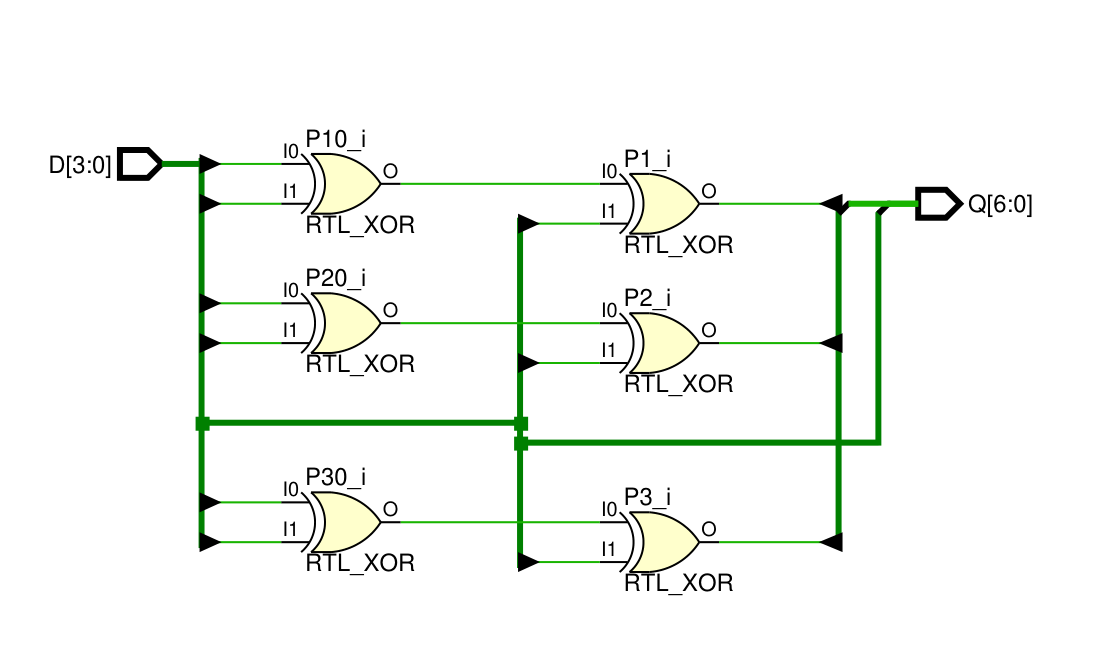
\includegraphics[scale=.55]{examp121}
	\caption{Synthesized Parity Checker}
\end{figure}

\begin{examp}
	\vspace{.5cm}
	\textbf{The ALU Reprise}\\
	\begin{TermUnix}{hbox}
		library IEEE;
		use IEEE.std_logic_1164.all;
		use IEEE.numeric_std.all;

		entity ALU2ElectricBoog is

		port(
		B	: in	std_logic_vector(1 downto 0);
		A	: in	std_logic_vector(1 downto 0);
		Q	: out	std_logic_vector(3 downto 0);
		Op	: in	std_logic_vector(1 downto 0)
		);

		end ALU2ElectricBoog;

		architecture arch1 of ALU2ElectricBoog is
		begin
		process (A, B, Op)
		begin
		if Op = "00" then
		Q <= "00" & A and "00" & B;
		elsif Op = "01" then
		Q <= "00" & A or "00" & B;
		elsif Op = "10" then
		Q <= unsigned("00" & A) + unsigned("00" & B);
		elsif Op = "11" then
		Q <= unsigned(A) * unsigned(B);
		end if;
		end process;
		end arch1;

	\end{TermUnix}
	This assignment differed from the last by having the required portion be
	filled under the \texttt{process} block. Here, we define an operation that is
	similar to a MUX utilizing the \texttt{if-elsif} construct from VHDL.
	This is still using the \textit{behavioral} strategy of implementation with a
	\texttt{process} block.

	The explicit use of casting the unsigned type and concactenating the signals
	with leading \(00\) is explained further. The synthesized schematic is as
	follows:
	\begin{figure}[H]
		\centering
		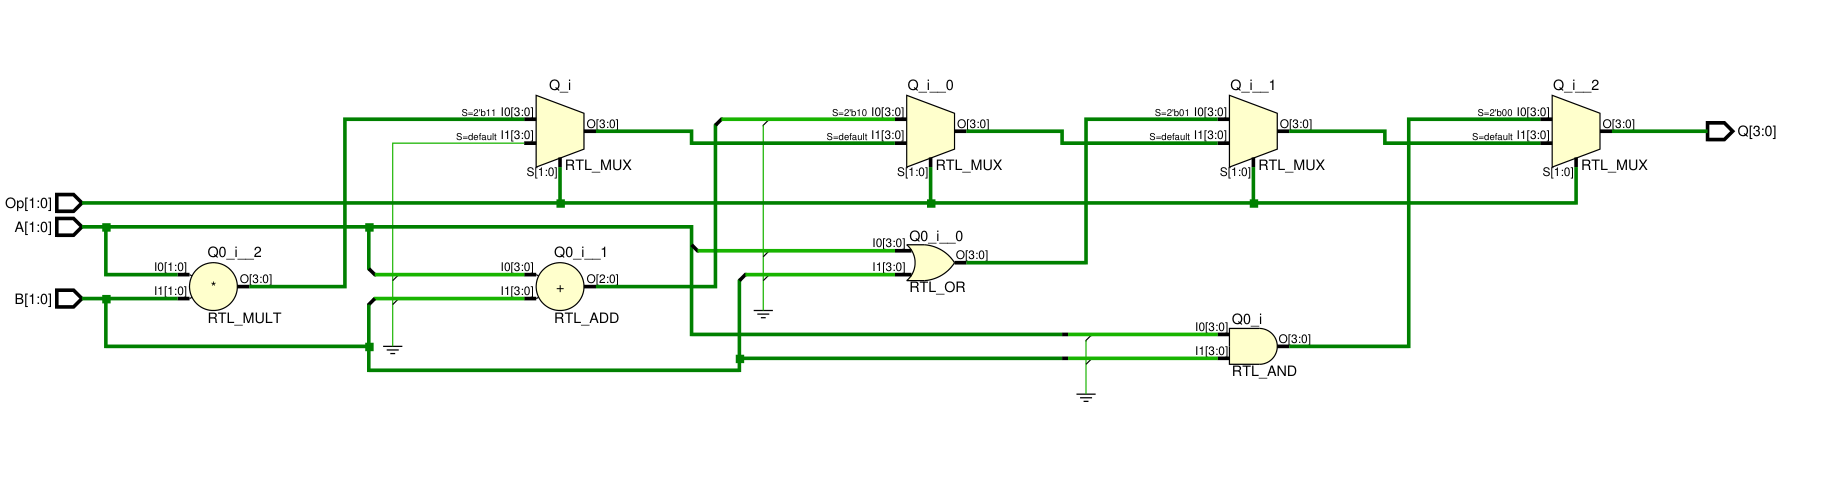
\includegraphics[scale=.35]{examp122}
		\caption{Synthesized Toy ALU}
	\end{figure}
\end{examp}
\begin{examp}
	\vspace{.5mm}
	\subsubsection*{The Use of \texttt{unsigned()} Cast}
	The \texttt{unsigned()} function in VHDL is used to cast a binary vector to an \texttt{UNSIGNED} type, treating the vector as a positive integer. This explicit casting allows VHDL to interpret binary data without ambiguity, particularly during arithmetic operations, ensuring that the result is processed as an unsigned value. In VHDL, operations between \texttt{SIGNED} and \texttt{UNSIGNED} types require conversions to maintain compatibility, as VHDL does not implicitly mix these types.

	\textbf{\texttt{unsigned()}} ensures that \texttt{A} and \texttt{B} are interpreted as positive integers, allowing for correct behavior in operations like addition (\texttt{+}) without treating them as potentially negative numbers.

\end{examp}
\begin{examp}
	\subsubsection*{Effect of Using \texttt{signed()} Instead of \texttt{unsigned()}}

	If you were to replace \texttt{unsigned()} with \texttt{signed()} in the ALU, the output could change significantly, particularly in cases where \texttt{A} or \texttt{B} have high bits set to \texttt{1} (interpreted as negative in 2’s complement). For example:
	\begin{itemize}
		\item With \textbf{\texttt{unsigned}}, a binary vector such as \texttt{"1100"} would be interpreted as \(12\).
		\item With \textbf{\texttt{signed}}, the same vector \texttt{"1100"} would be interpreted as \(-4\) in 2's complement form.
	\end{itemize}


	This change would result in different outputs for operations that involve addition or multiplication, where the result might switch from a positive to a negative value, depending on the high bits of the input.
\end{examp}
\begin{examp}

	\subsubsection*{Circuit Element Emulated by \texttt{if} and \texttt{elsif} Statements}
	In the ALU, the \texttt{if} and \texttt{elsif} statements emulate the behavior of a \textbf{multiplexer (MUX)}. The \texttt{Op} input acts as a selector that determines which operation (AND, OR, ADD, or MULTIPLY) the ALU will perform based on its value. Each condition (e.g., \texttt{Op = "00"}, \texttt{Op = "01"}, etc.) corresponds to a specific operation, similar to how a multiplexer selects an output based on control signals.

	In VHDL there are several other methods of defining a MUX like operation such
	as the use of the \texttt{when} and \texttt{else} operators.
\end{examp}

\begin{examp}
\subsubsection*{A Basic Combinational Logic Example}
A basic diagram is given that describes
\[
	Q = AB\closure{C} + A \oplus C
\]
To create this in a VHDL simulation, the following behavioral entity is
employed:
\begin{TermMac}{hbox}
library IEEE;
use IEEE.std_logic_1164.all;
use IEEE.numeric_std.all;

entity examp6 is
port (
A, B, C : in std_logic;
Q : out std_logic
);
end examp6;

architecture rtl of examp6 is
begin
Q <= (A and B and (not C)) or (A xor C);
end rtl;
\end{TermUnix}

This highlights how simple it is to assign complex combinational statements in
a synthesizeable form.

\begin{figure}[H]
	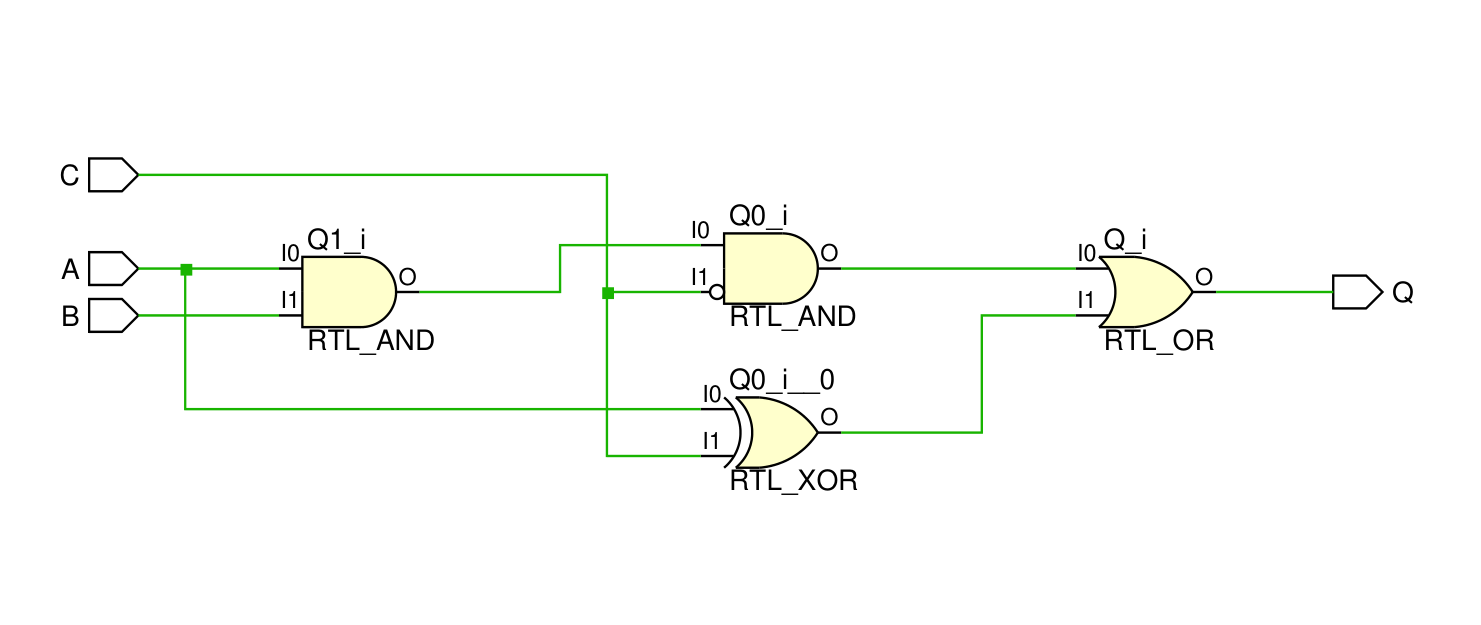
\includegraphics[scale=.45]{examp123}
	\caption{Synthesized Schematic from VHDL}
\end{figure}

\end{examp}
\begin{examp}
	\subsubsection*{Another Multiplexor Example}
	As stated before, a MUX can be employed in VHDL in several different ways.
	This goes back to utilizing the \texttt{if-elsif} operators, which are
	straight forward to implement.

	A 4 input MUX with a 2 bit selector is shown
	that uses two inputs, $A$ and $B$ to implement some sort of logical operation
	which as seen in previous labs, could be used to implement a larger machine
	such as a 12-person voting machine.

	Since we only write synthesizeable VHDL here and not other silly business, the
	code is completed as follows:
	\begin{TermUnix}{hbox}
		library IEEE;
		use IEEE.std_logic_1164.all;

		entity examp7 is
		port (
		sel : in std_logic_vector(1 downto 0);
		A, B : in std_logic;
		Q : out std_logic
		);
		end examp7;

		architecture rtl of examp7 is
		begin
		process (A, B, sel)
		begin
		if sel = "00" then
		Q <= '0';
		elsif sel = "01" then
		Q <= A and B;
		elsif sel = "10" then
		Q <= A;
		elsif sel = "11" then
		Q <= B;
		else
		Q <= '0';
		end if;
		end process;
		end rtl;
	\end{TermUnix}
	This example is slightly more challenging due to the careful use of the
	\texttt{""} operators and the required formatting for each line according to
	the VHDL standard.

	To ensure clarity and adherence to best practices, it is customary to write
	processes like this for readability. For example, consider the statement:
	\begin{verbatim}
Q <= '0';
        \end{verbatim}
	In this case, \texttt{Q} is of type \texttt{std\_logic}, while \texttt{sel} is
	of type \texttt{std\_logic\_vector}. The assignment utilizes the \texttt{''}
	operators which are subtly different than the ones employed the line prior.
	This distinction is crucial because
	attempting to assign a \texttt{std\_logic\_vector} directly to a
	\texttt{std\_logic} would result in errors. This subtle type
	mismatch is a common source of bugs and can lead to hours of troubleshooting if
	not addressed early. (Ask me how I know!)

	Additionally, the assignment code excluded something very important for
	synthesis, a default condition for the \texttt{sel} utilizing a terminating
	\texttt{else}. Without this, undesired outcomes may occur during synthesis as
	the software would place a latch on the output of the circuit, which is not
	what is intended. I have included this in my code above and assigned Q a 0 for
	all other edge cases. Again, this might not be pertinent to such a simple
	design, but can result in nasty, nasty bugs in the testbench.
	\begin{figure}[H]
		\centering
		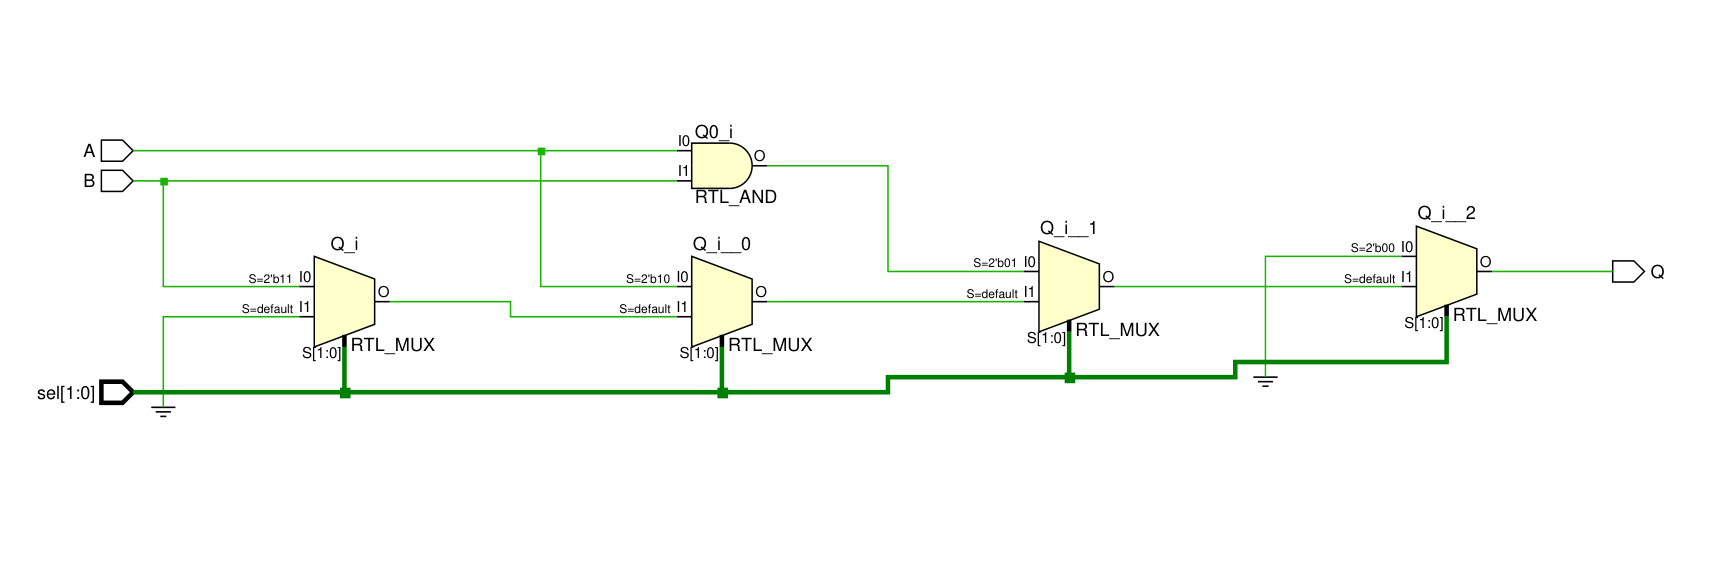
\includegraphics[scale=.35]{examp124}
		\caption{Synthesized Mux Module from VHDL}
	\end{figure}
\end{examp}
\end{document}
